% vim: set tw=78 tabstop=4 shiftwidth=4 aw ai:

\chapter{Designing an Improved Multiparty Protocol in the Linux Kernel}
\label{chapter:multiparty}

\section{The swift Multiparty Protocol}
\label{sec:multiparty:swift}

The \textit{swift} protocol is a generic multiparty transport protocol. Its
mission is to disseminate content among a swarm of peers. Basically, it
answers one and only one request: \textit{'Here is a hash! Give me data for
it!'}. Such entities as storage, servers and connections are abstracted and
are virtually invisible at the API layer. Given a hash, the data is received
from whatever source available and data integrity is checked cryptographically
with Merkle hash trees~\cite{merkle}.

Most features of the \textit{swift} protocol are defined by its function as a
content-centric multiparty transport protocol. A significant difference
between \textit{swift} and the TCP protocol is that TCP possesses no
information regarding what data it is dealing with, as data is passed from
user-space, while the \textit{swift} protocol has data fixed in advance
and many peers participate in distributing the same data. Because of this and
the fact that for \textit{swift} the order of delivery is of little importance
and unreliability is naturally compensated for by redundancy, it entirely
drops TCP's abstraction of sequential reliable data stream delivery. For
example, out-of-order data could still be saved and the same piece of data
might always be received from another peer.

Our main objective is to integrate \textit{swift} as a transport protocol in
the Linux kernel networking stack. This will provide notable performance
improvement regarding data transfer. We intend to do this with minimal
intrusion effect in the Linux kernel and also to change as little as possible
the current \textit{swift} implementation. Another goal is to provide a
transparent API between the kernel and the user space. A developer will use a
socket-like interface when building an application on top of the
\textit{swift} protocol. In order to achieve this goal we have implemented an
intermediary step. We have simulated the kernel part in the user-space using
raw sockets. This has the advantage of providing means to have modular
functionality tests.

\section{Designing a Multiparty Protocol}
\label{sec:multiparty:design}

While designing our system, we have tackled a few different ideas, each with
its strengths and weaknesses. We present some of those preliminary ideas
that lead to the our current desing choice.

The first approach we thought of was to include all of the swift protocol into
kernel space. This approach had the advantage of simplicity and would have
implied minimal architectural changes. The current user space implementation
could have been ported to a kernel module.

Though simple, this approach could not be implemented because of the
restriction of memory size in the kernel.  For the integrity check the swift
protocol relies on Merkle hash tree. Keeping this tree in the kernel space
memory is not scalable. The Internet content is too large to be stored in
kernel space. Even if the tree retains only hashes of the data disseminated, the
space is insufficient.

\section{Raw Socket Wrapper Implementation}
\label{sec:multiparty:raw-socket}

\subsection{Raw Socket-Based Architecture}

In figure Figure~\ref{fig:multiparty:architecture-overview} we see the main
conceptual modules: Application module, wrapper library, peer discovery
overlay and the swift transport protocol layer.

\begin{figure}
  \centering
  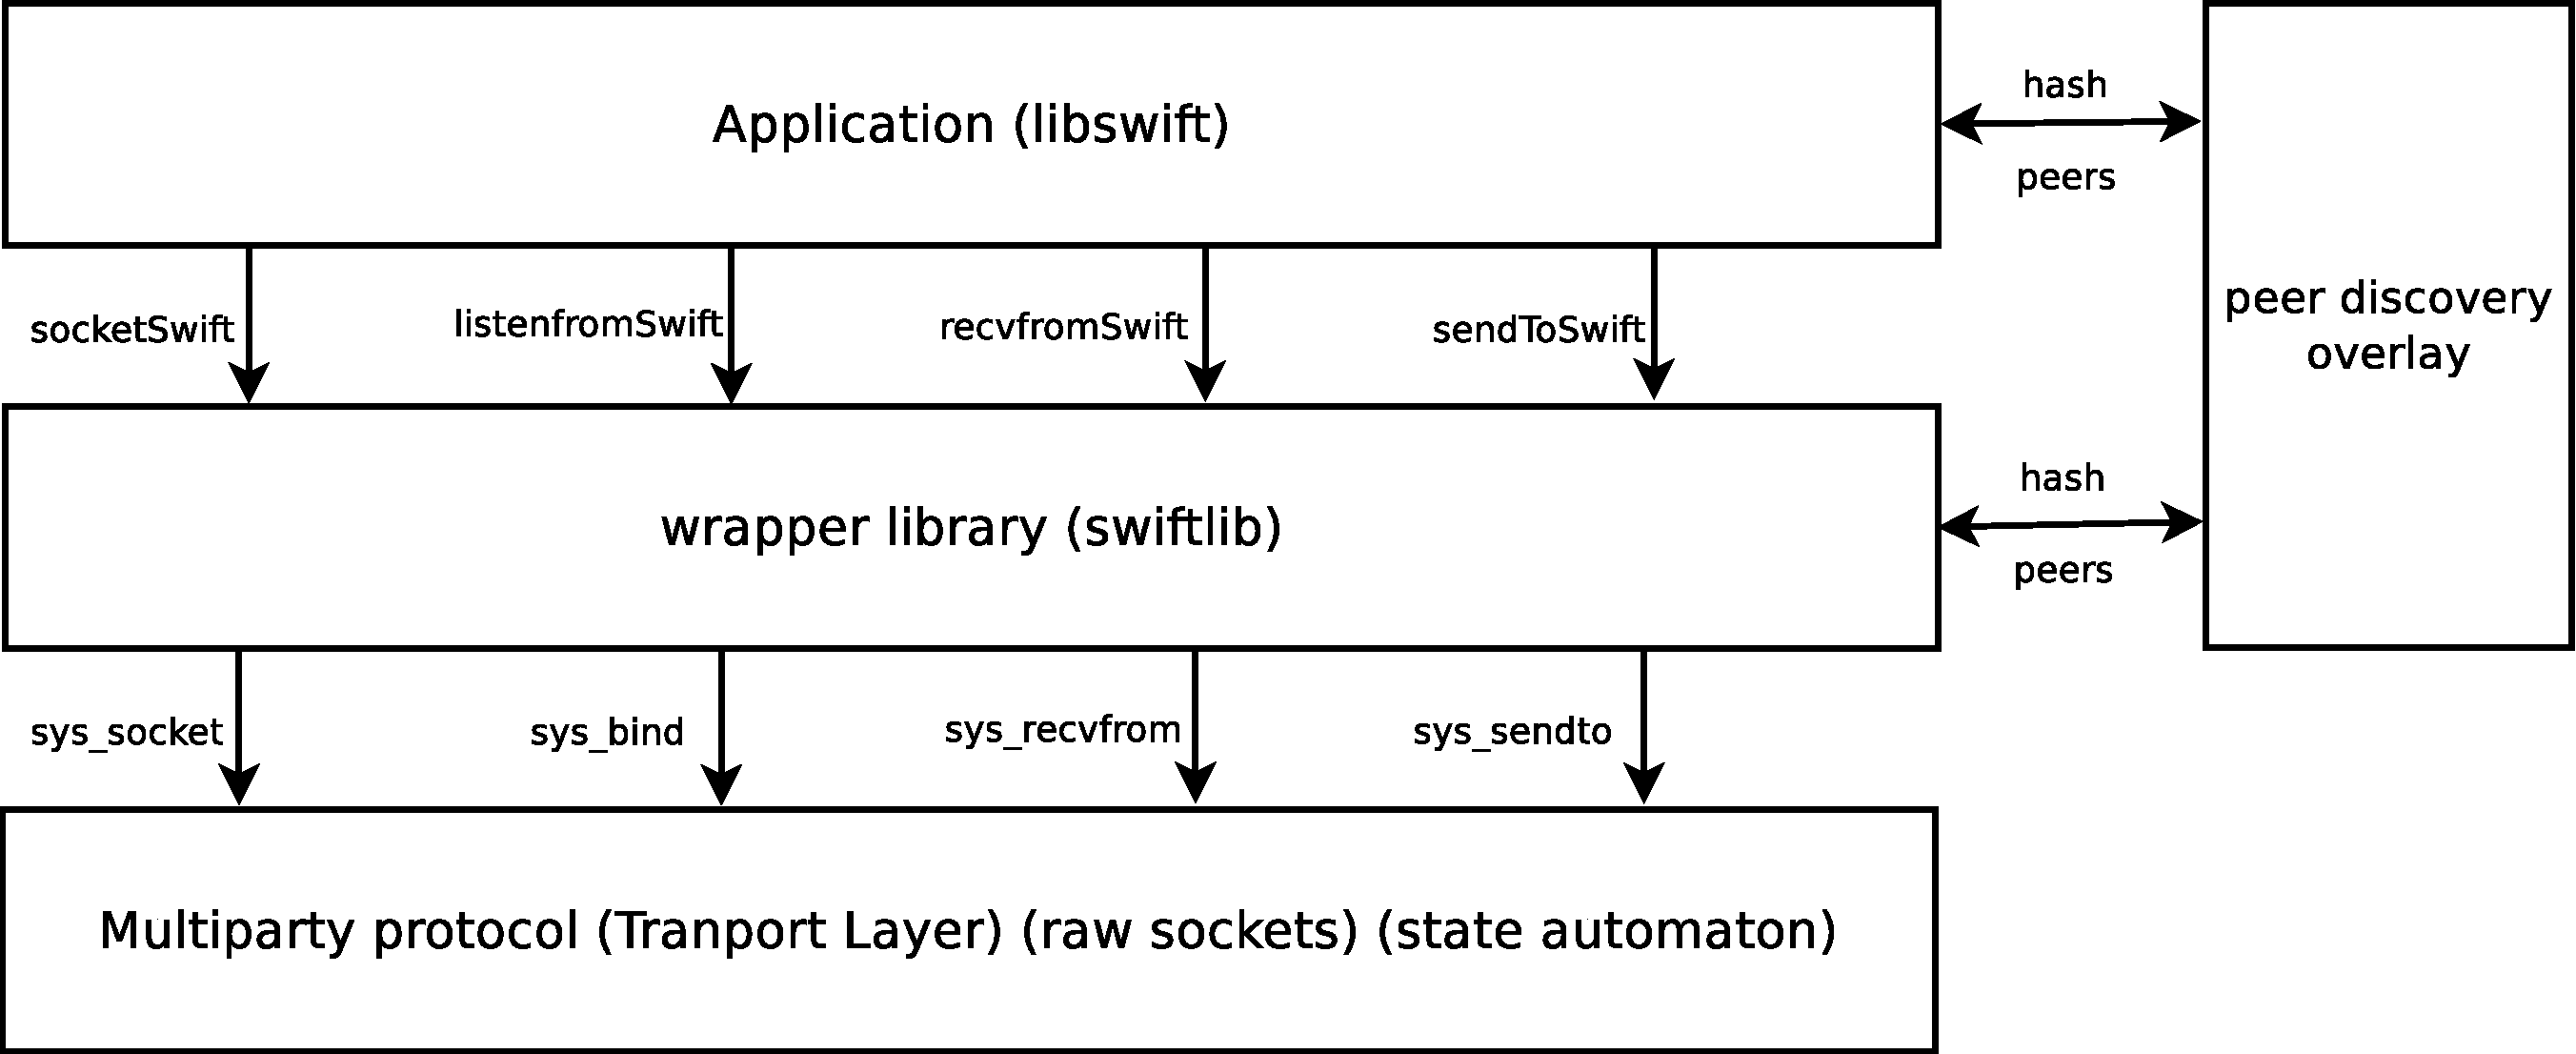
\includegraphics[width=0.6\textwidth]{src/img/multiparty/architecture-overview}
  \caption{Overview Architecture}
  \label{fig:multiparty:architecture-overview}
\end{figure}

The Application module represents the remaining part of the old swift
implementation. This is the part that remains in user space and contains the
file management and hash management features. 

The wrapper library module defines a socket-like API for the user space
applications. A regular program will use those calls instead of the normal
socket ones to use the multiparty sockets. For the moment those calls are
simulated system calls that initially are resolved with the socket raw
implementation (still in user space). In the future this wrapper library
will represent entry points into the kernel.

The peer discovery overlay will remain unchanged. It is still going to work
based on UDP sockets and link the same levels in the swift implementation as
before. The peer discover will be part of the application implementation and
it will be the developer's choice how to implement and how to manage it.

The multiparty protocol is implemented for now at user space level through a raw
socket layer to validate our architecture. This has the advantage of
simulating the real design modularization but also permits an easier debugging
and testing procedure of the integration. In the next step this part will be
represented by a kernel patch that will communicate through custom made system
calls with the wrapper library. This two phases are described in
Figure~\ref{fig:multiparty:detailed-architecture}.

\begin{figure}
  \centering
  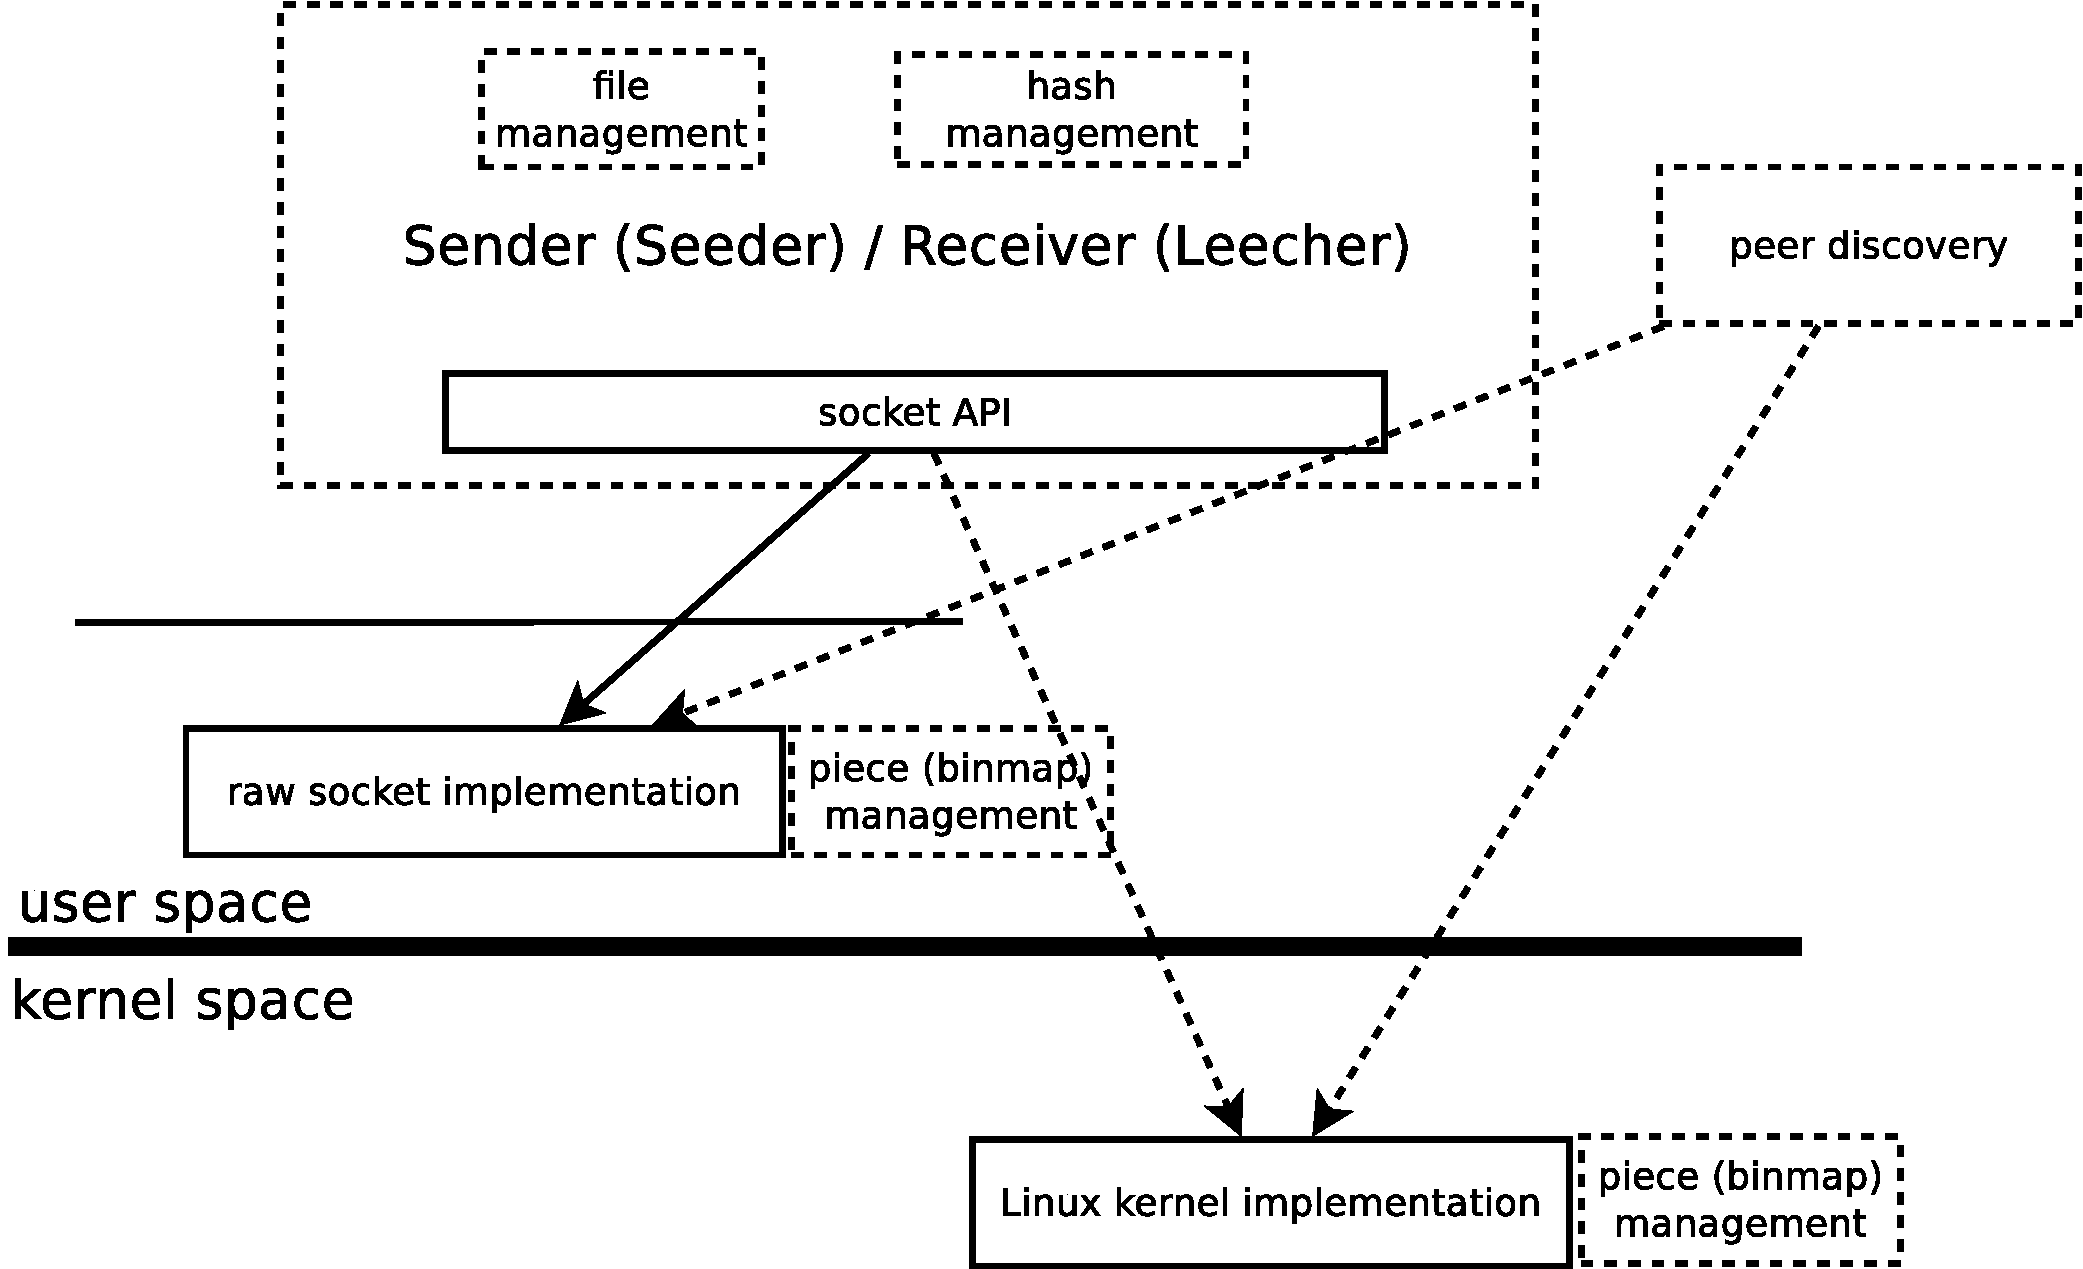
\includegraphics[width=0.6\textwidth]{src/img/multiparty/detailed-architecture}
  \caption{Detailed Architecture}
  \label{fig:multiparty:detailed-architecture}
\end{figure}

\begin{figure}
  \centering
  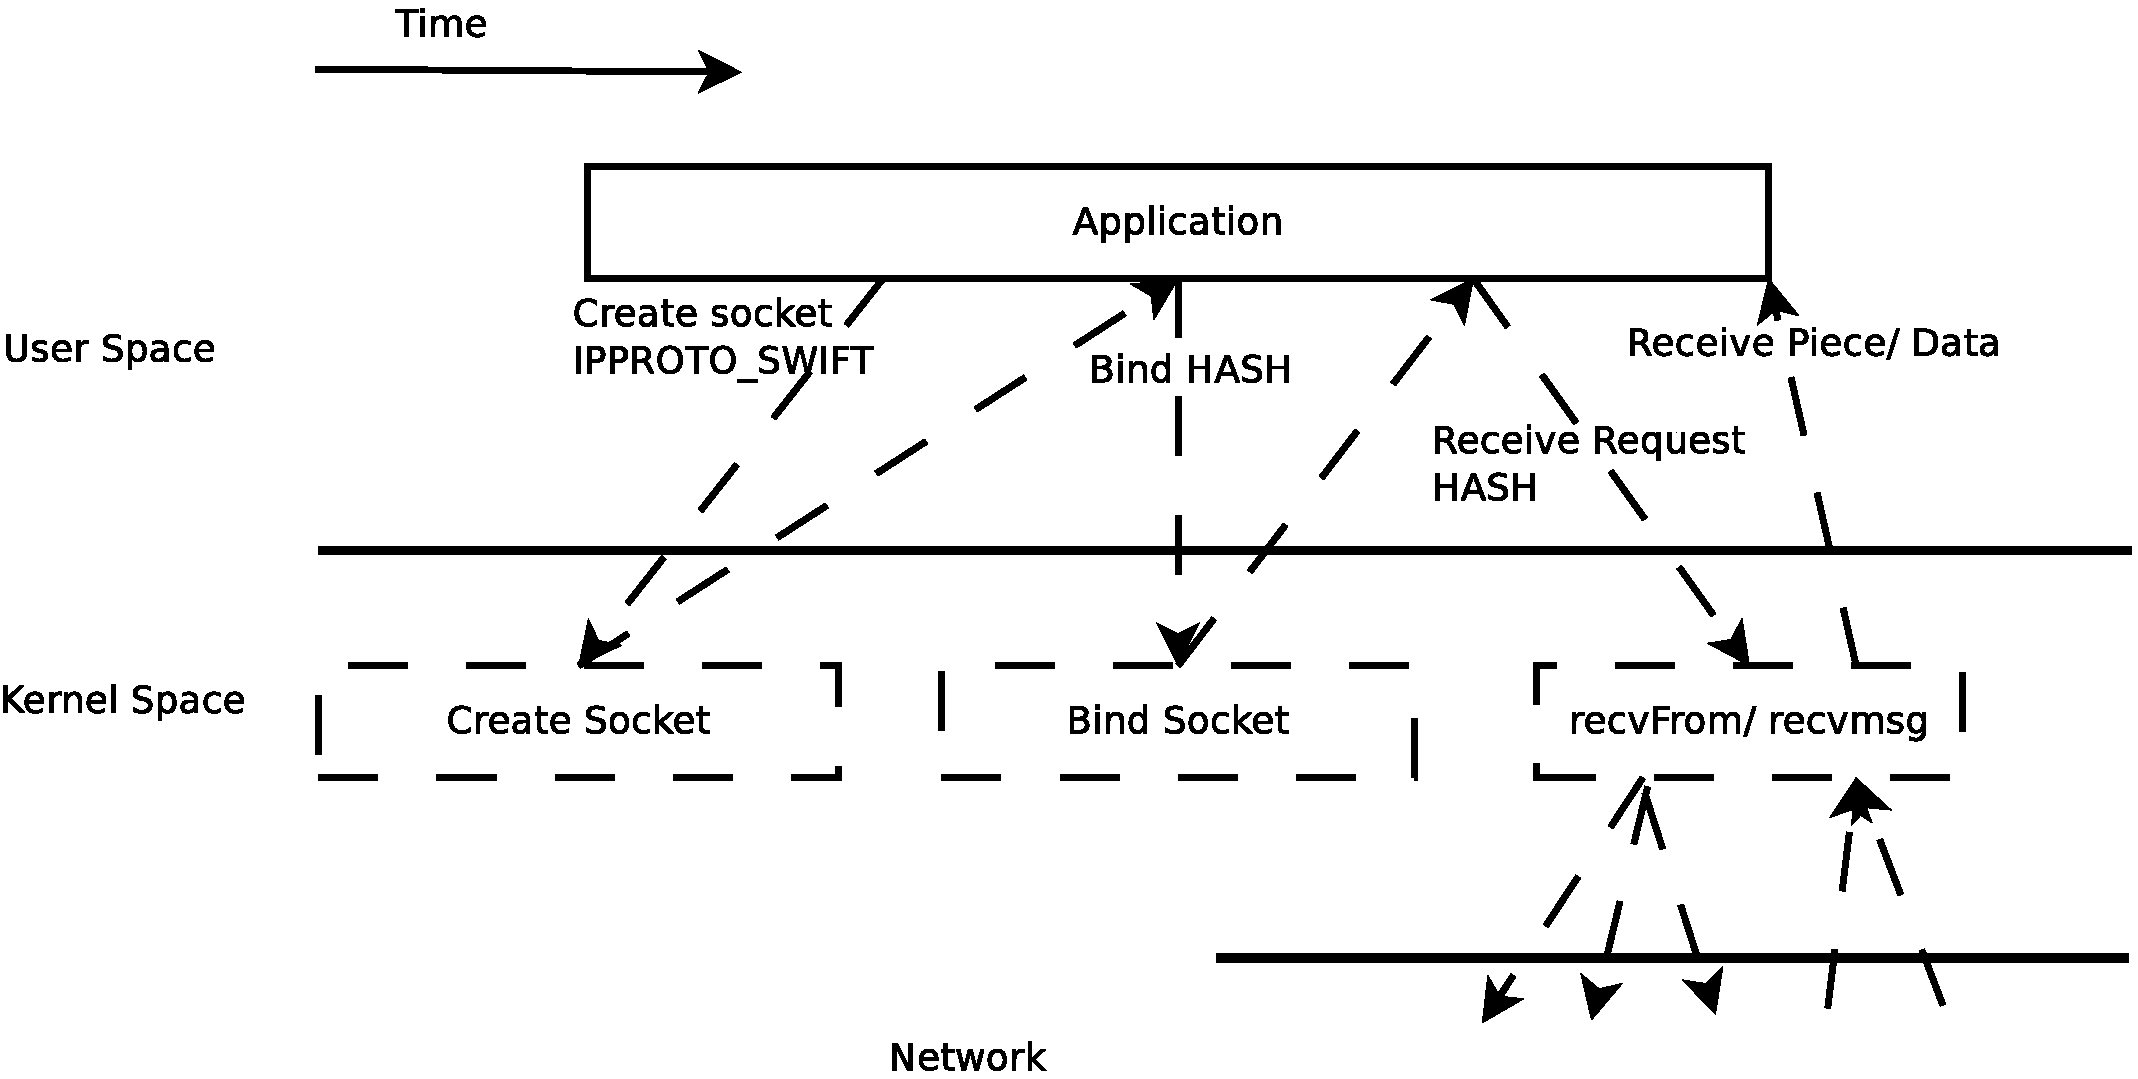
\includegraphics[width=0.55\textwidth]{src/img/multiparty/multiparty-recvmsg}
  \caption{Receiver Conceptual Model}
  \label{fig:multiparty:multiparty-recvmsg}
\end{figure}

Figure~\ref{fig:multiparty:multiparty-recvmsg} presents the conceptual model
of the Leecher. The Leecher is the one that requests data data. In order
to do this it must connect to the multiparty protocol by creating and binding
to a multiparty socket. When it binds to a socket, it uses the hash as a
parameter to find a connection with a peer that accesses the respective file.
This discovery is done through the separate peer discovery overlay. The
Leecher then waits for packets from seeders.

\begin{figure}
  \centering
  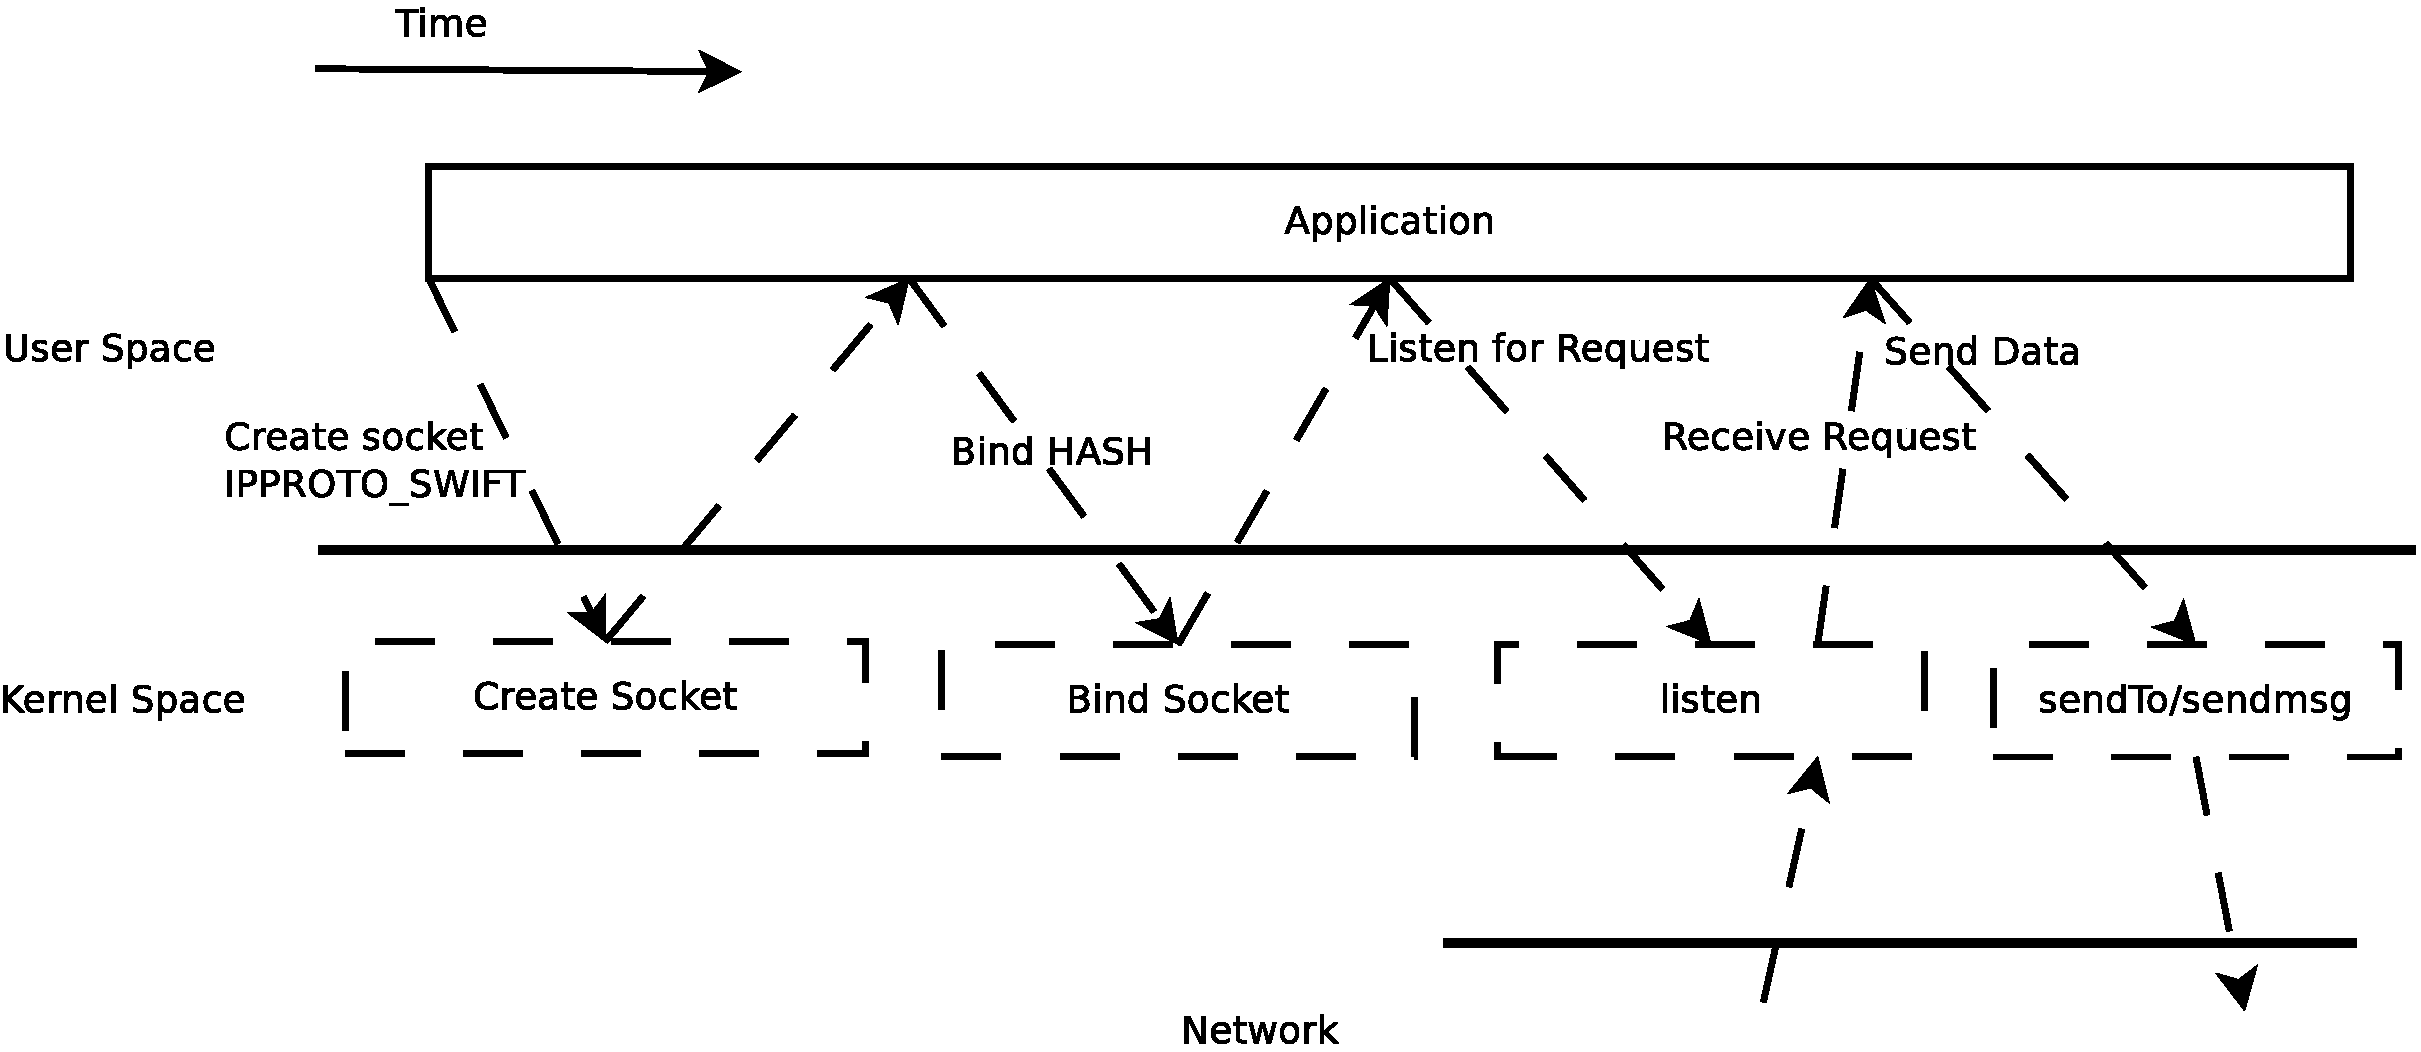
\includegraphics[width=0.55\textwidth]{src/img/multiparty/multiparty-sendmsg}
  \caption{Sender Conceptual Model}
  \label{fig:multiparty:multiparty-sendmsg}
\end{figure}

Figure~\ref{fig:multiparty:multiparty-sendmsg} presents the conceptual model
of the Seeder. The Seeder is the one that serves data to other Leechers. In
order to do this it must connect to the multiparty protocol by creating,
binding and listening to a multiparty socket. When binding, the Seeder
uses the hash as a parameter. This means that for every file hashed there will
be a socket on which the seeder that may receive and serve requests. The Seeder
then waits for requests and sends data packets as requested.

\subsection{Testing of Raw Socket Implementation}

The  protocol is a generic multiparty transport protocol. Its mission is to
disseminate content among a swarm of peers.  Given a hash, the data is
received from whatever source available and data integrity is checked
cryptographically with Merkle hash trees. 

Our main focus when modifying the swift implementation is to have an impact on
time performance. With a communication protocol the greatest latency is
usually generated by waiting for the results from the network. The multiparty
communication model already takes care of this, so the next best thing is to
enhance the application time. We are doing this by decreasing time
penalties due to context switches between user space and kernel space. The
main idea is to reduce the number of system calls made from user space into
the kernel. This implicitly reduces the number of preemption moments.

First, we have implemented a test suite for every socket system call, which
tests all possible cases. These unit tests are created to ensure the code
quality, and to validate if the system call behave in the same mode as other
similar system call.

Secondly, we have implemented a functional test suite to validate a simple
workflow. For this purpose we tested a peer that acts as the seeder and a
receiver which behaves as a leecher. A small file is transfered between the
two entities to ensure proper delivery.

The test suite is mainly implementing using arrays of function pointers or
function pointer structures. A top level structure defines test suites for
each function exported by the implementation. Each test suite is a series of
methods that test a variant of the call of the function.

\section{Kernel Framework for Multiparty Protocol Implementation}
\label{sec:multiparty:kernel-framework}

The introduction of a multiparty protocol in the Linux kernel was a challenge,
because of its particularities versus common protocol implementations. A
multiparty transport protocol uses multiple points in a communication, unlike
a traditional communication protocol that allows a sender endpoint and a
receiver endpoint.

\subsection{Transport Protocol Implementation on the Linux Kernel}

In order to implement o transport protocol in the Linux kernel, several design
phases must be established:

\begin{itemize}
  \item Defining \texttt{IPPROTO\_\$\$}. This macro will identify the
  transport protocol. This will be subsequently used for creating a transport
  protocol socket.
  \item Defining a transport header. The framework we used defined two 8 bit
  ports, a source port and a destination port and a 16 bit lenght field. The
  latter field is the data length, including the tranport protocol header.
\end{itemize}

After the above have been completed, several data structures have to be
defined, as mentioned below.

A data structure that defines the new socket type. This is where we must save
information regarding the socket state, such as the destination or the source
port.
\begin{verbatim}
struct swift_sock {
    struct inet_sock sock;
    /* swift socket speciffic data */
    uint8_t src;
    uint8_t dst;
};
\end{verbatim}

The protocol definition, used by the socket, including its name and size are
defined in a \texttt{struct proto} structure.
\begin{verbatim}
static struct proto swift_prot = {
    .obj_size = sizeof(struct swift_sock),
    .owner = THIS_MODULE,
    .name = "SWIFT",
};
\end{verbatim}

The most important structure to be defined describes the operations that are
supported by a socket of a given type. For a datagram sending socket, the
implementation of \texttt{release}, \texttt{connect}, \texttt{sendmsg} and
\texttt{recvmsg} functions is sufficient.

The new packtets header are setup in the \texttt{net\_protocol} header. New
packets that are received directly from the network will fill the
\texttt{protocol} field in the IP header with the value of the implemented
Transport Level protocol.

Before compiling and inserting the module in the kernel, several socket
operations functions have to be filled; for swift (a datagram based protocol),
this would mean \texttt{release}, \texttt{bind}, \texttt{connect},
\texttt{sendmsg} and \texttt{recvmsg}. A handler for packets received from the
network must also be implemented. At protocol level, one must keep a mapping
between a port and a socket, meaning that the socket is bound to that port.

\subsection{Testing the Kernel Protocol Implementation}

Unit tests have been employed for testing the protocol. Among those are a few
simple tests, to ensure basic functionality and then a set of new tests that
check error codes and protocol performance. Protocol performance is related to
ensuring scalability -- multiple simulateneous client connections.

Basic functional testing means the design and implementation of tests for each
function exposed by the protocol. That is, there is a given test for each of
\texttt{bind}, \texttt{connect}, \texttt{close}, \texttt{sendto},
\texttt{recvfrom}, \texttt{sendmsg}, \texttt{recvmsg}, \texttt{send} and
\texttt{recv}. The test suite is used is the same one used for the raw
socket implementation. Due to the identical API provided, we could easily use
those test for the kernel implementation.

Negative testing, for unwanted/unwelcome situations is similarly accomplished:
each function exposed by the protocol is assigned a test. For example, the
\texttt{bind} system call will always check an error being returned for a
duplicate call using the same port. As is the case for the use of invalid IP
addresses or invalid port numbers. A series of such tests will be employed for
each functionality.

Performance testing is completed through the use of multiple protocol sockets.
Data sent from the socket is checked against data arriving at the other
end; this actually means checking whether port and socket mapping is working
according to the specifications. Another measure of protocol performance is
the transfer speed on the newly created socket.
